\chapter{Số học}

\epigraph{{\rmfamily Toán học là vua của các môn khoa học, và số học là nữ hoàng}}{Carl Friedrich Gauss}

\begin{figure}[ht]
    \centering
    \fbox{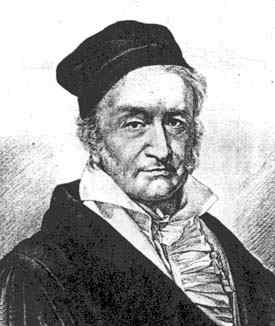
\includegraphics{mathematicians/Gauss.jpeg}}
    \captionsetup{labelformat=empty}
    \caption{Carl Friedrich Gauss (1777-1855)}
\end{figure}

\section{Phép chia Euclid và thuật toán Euclid}

\subsection*{Phép chia Euclid}

Đây là nền tảng, cơ sở của số học. Từ khi biết tới phép chia hai số nguyên, ta có thể tìm \textit{thương} và \textit{số dư}. Nói theo toán học, nếu ta có hai số nguyên dương $a$ và $b$ thì tồn tại cặp số $q$, $r$ sao cho $a = qb + r$ với $0 \leqslant r < b$.

Khi đó, $a$ gọi là số bị chia, $b$ gọi là số chia, $q$ là thương (q trong quotient) và $r$ là số dư (r trong remainder).

Đặc biệt là sự tồn tại của cặp số $q$ và $r$ là duy nhất. Thật vậy, nếu ta giả sử tồn tại 2 cặp số $(q_1, r_1)$ và $(q_2, r_2)$  đều thỏa đẳng thức trên, nghĩa là
\[a = q_1 b + r_1, \quad a = q_2 b + r_2\]

Trừ 2 đẳng thức vế theo vế ta có $(q_1 - q_2) b + (r_1 - r_2) = 0$. Tương đương $(r_2 - r_1) = (q_1 - q_2) b$, mà $0 \leqslant r_1, r_2 < b$ nên $-b < r_2 - r_1 < b$. Như vậy chỉ có thể xảy ra trường hợp
$r_2 - r_1 = 0$ hay $r_2 = r_1$, kéo theo $q_1 = q_2$.

\subsection*{Thuật toán Euclid}

Dựa trên phép chia Euclid, ta có một thuật toán hiệu quả để tìm ước chung lớn nhất giữa hai số $a$ và $b$.

Ký hiệu $\gcd(a, b)$ là ước chung lớn nhất của $a$ và $b$. Chúng  ta thực hiện đệ quy như sau:
\begin{equation*}
    \gcd(a, b) = \begin{cases}
        a, \quad & \text{nếu}\,b = 0 \\
        \gcd(b, a \bmod b), \quad & \text{nếu}\,b \neq 0
    \end{cases} 
\end{equation*}

Điểm quan trọng ở thuật toán Euclid là thuật toán chắc chắn sẽ dừng sau một số hữu hạn bước, và kết quả sẽ là ước chung lớn nhất của hai số $a$ và $b$.

\begin{proof}
    Đặt $r_0 = a$ và $r_1 = b$. Theo thuật chia Euclid ta có các số $q_0$ và $r_2$ sao cho $r_0 = r_1 q_0 + r_2$ với $0 \leqslant r_2 < r_1$. Thuật toán Euclid hoạt động như sau:
    \begin{align*}
        r_0 & = r_1 q_0 + r_2 \\
        r_1 & = r_2 q_1 + r_3 \\
        r_2 & = r_3 q_2 + r_4 \\
        \ldots & = \ldots \\
        r_i & = r_{i+1} q_i + r_{i+2} \\
        \ldots & = \ldots \\
        r_k & = r_{k+1} q_k + 0 \\
        r_{k+1} & = 0
    \end{align*}
    Ta thấy rằng ở mỗi bước, $r_{i+2}$ luôn nhỏ hơn $r_{i+1}$. Do đó cuối cùng sẽ bằng 0, và khi đó ta có ước chung lớn nhất.
\end{proof}

\subsection*{Thuật toán Euclid mở rộng}

\begin{definition}[Phương trình Diophantos]
    Cho trước các số nguyên $a$, $b$ và $c$. Phương trình  Diophantus là phương trình có dạng
    \[ax + by = c\]
    với $x$, $y$ là các số nguyên.
\end{definition}

\begin{example}
    Giải phương trình $5x+3y = 1$.

    Ta có $y = \dfrac{1-5x}{3} = \dfrac{1-2x-3x}{3} = \dfrac{1-2x}{3} - x$. Như vậy nếu $y \in \ZZ$ thì $\dfrac{1-2x}{3} \in \ZZ$, nghĩa là $1-2x$ chia hết cho 3. Vậy $1-2x = 3k$ với $k \in \ZZ$.

    Tiếp tục, $1-2x = 3k$, suy ra $x = \dfrac{1-3k}{2}  = \dfrac{1-k-2k}{2} = \dfrac{1-k}{2} - k$. Do $x$ nguyên nên tương tự $\dfrac{1-k}{2}$ cũng nguyên, hay $1-k = 2t$, tương đương với $k = 1-2t$.

    Thay ngược lại ta có $x = \dfrac{1-3k}{2} = \dfrac{1-3(1-2t)}{2} = {-1+3t}$. Tiếp tục thay vào để tìm $y$ thì $y = \dfrac{1-5x}{3} = \dfrac{1-5(-1+3t)}{3} = 2 - 5t$.

    Như vậy nghiệm của phương trình là tất cả các nghiệm $(x, y)$ mà $x = -1+3t$, $y = 2-5t$ với $t \in \ZZ$.
\end{example}

Ở đây chúng ta đã thực hiện phép chia có dư liên tiếp để tìm nghiệm. Nói cách khác ta đã thực hiện thuật toán Euclid ở bên trên để làm giảm độ phức tạp ở mỗi bước giải. Tổng quát ta có thuật toán Euclid mở rộng để tìm ước chung lớn nhất $\gcd(a, b)$ của hai số $a$, $b$, và \textbf{một} nghiệm của phương trình $ax + by = \gcd(a, b)$.

Ở ví dụ trên, ta thấy rằng $(-1, 2)$ là một nghiệm của phương trình $5x + 3y = 1$. Khi đó ta có thể suy ra tất cả nghiệm (họ nghiệm) của phương trình có dạng $(-1+3t, 2-5t)$ với $t \in \ZZ$.

\begin{algorithm}
    \caption{Thuật toán Euclid mở rộng}
    \begin{algorithmic}
        \Require $a, b \in \ZZ$
        \Ensure $\gcd(a, b)$, $x$, $y$ 
        \State $r_0 \gets a$, $r_1 \gets b$, $r_2 \gets 0$
        \State $x_0 \gets 1$, $x_1 \gets 0$, $x_2 \gets 0$
        \State $y_0 \gets 0$, $y_1 \gets 1$, $y_2 \gets 0$
        \While{$r_1 \neq 0$}
            \State $q \gets r_0 \;\text{div}\; r_1$
            \State $r_2 \gets r_0 - q * r_1$, $r_0 \gets r_1$, $r_1 \gets r_2$
            \State $x_2 \gets x_0 - q * x_1$, $x_0 \gets x_1$, $x_1 \gets x_2$
            \State $y_2 \gets y_0 - q * y_1$, $y_0 \gets y_1$, $y_1 \gets y_2$
        \EndWhile
        \State \Return $r_0$, $x_0$, $y_0$
    \end{algorithmic}
\end{algorithm}

Ở thuật toán trên, $r_0$, $r_1$ và $r_2$ hoạt động như thuật toán Euclid chuẩn. Ở mỗi bước $q$ là thương của phép chia hai số nguyên và ta sử dụng $q$ đó để tính $x_0$ và $y_0$ mới. Kết quả cuối cùng $(r_0, x_0, y_0)$ lần lượt là ước chung lớn nhất, và hai số $x$, $y$ thỏa mãn $a x_0 + y b_0 = r_0$.

Tại sao chúng ta lại có $(x_0, x_1) = (1, 0)$ và $(y_0, y_1) = (0, 1)$? Nói cách khác, làm sao biết thuật toán  hoạt động đúng?

Mục đích của chúng ta là tìm các số $(x, y)$ sao cho $ax + by = \gcd(a, b)$. Khi đó, dựa trên thuật toán Euclid cơ bản ở trên, ta xây dựng dãy số $\{x_n\}$ và $\{y_n\}$ sao cho ở mọi bước thứ $n$ ta đều có

\begin{equation}\label{euclid:1}
    a x_n + b y_n = r_n
\end{equation}

Ta có $r_i = r_{i+1} q_i + r_{i+2}$. Từ $q_i$ ở mỗi bước ta tính được
\begin{equation*}
    x_i = x_{i+1} q_i + x_{i+2}, \quad y_i = y_{i+1} q_i + y_{i+2}
\end{equation*}

Thay vào \ref{euclid:1} ta được
\begin{equation}
    a (x_{i+1} q_i + x_{i+2}) + b (y_{i+1} q_i + y_{i+2}) = r_i
\end{equation}

Tương đương với \[(a x_{i+1} + b y_{i+1}) q_i + (a x_{i+2} + b x_{i+2}) = r_i\]

Mà $a x_{i+1} + b y_{i+1} = r_{i+1}$ và $a x_{i+2} + b y_{i+2} = r_{i+2}$. Suy ra $r_{i+1} q_i + r_{i+2} = r_n$, đúng với thuật toán Euclid chuẩn ban đầu. Nghĩa là thuật toán hoạt động đúng. Bây giờ ta cần chọn $(x_0, x_1)$ và $(y_0, y_1)$ vì chúng ta đã đặt $r_0 = a$ và $r_1 = b$. Ở bước thứ 0, \[r_0 = a = a x_0 + b y_0\] và ở bước thứ 1,
\[r_1 = b = a x_1 + b y_1\]

Dễ thấy ở bước 0 ta chọn $(1, 0)$ và ở bước 1 ta chọn $(0, 1)$ là được.

\section{Hàm Euler}

\begin{definition}[Phi hàm Euler]
    Cho số nguyên dương $n$. Số lượng các số dương nhỏ hơn $n$ và nguyên tố cùng nhau với $n$ được ký hiệu bởi $\phi(n)$ và gọi là $\phi$ hàm Euler. \[ \phi(n) = \lvert \{ a : (a, n) = 1\} \rvert \]
\end{definition}   

Hàm Euler có ý nghĩa quan trọng trong lý thuyết số, công cụ giúp chúng ta giải các vấn đề về số mũ trong modulo.

Sau đây chúng ta xem xét hệ thặng dư đầy đủ và hệ thặng dư thu gọn.

Với số nguyên dương $n$, ta định nghĩa

\begin{definition}[Hệ thặng dư đầy đủ]
    Hệ thặng dư đầy đủ của $n$ là tập $\{0, 1, \ldots, n-1\}$.
\end{definition}

Nói cách khác, hệ thặng dư đầy đủ của $n$ là các số dư có thể có khi chia một số bất kì cho $n$.

\begin{definition}[Hệ thặng dư thu gọn]
    Hệ thặng dư thu gọn của $n$ là tập các số $a$ mà $1 \leqslant a < n$ và $(a, n) = 1$. Số lượng các số $a$ như vậy là $\phi (n)$.  
\end{definition}

\begin{remark}
    \begin{enumerate}
        \item Hệ thặng dư thu gọn của $n$ gồm $\phi(n)$ phần tử là \[ \{a_1, a_2, \ldots, a_{\phi(n)}\} \]
        \item Nếu $n$ là số nguyên tố thì $\phi(n) = n-1$.
    \end{enumerate}
\end{remark}

\subsection*{Tính chất hàm Euler}

\begin{remark}
    Với $(m, n) = 1$ thì $\phi(m n) = \phi(m) \phi(n)$.
\end{remark}

\begin{proof}
    Ta viết các số từ 1 tới $mn$ thành bảng như sau

    \begin{table}
        \centering
        \begin{tabular}{c c c c}
            1 & $m+1$ & $\cdots$ & $(n-1)m + 1$ \\
            2 & $m+2$ & $\cdots$ & $(n-1)m + 2$ \\
            $\cdots$ & $\cdots$ & $\cdots$ & $\cdots$ \\
            $m$ & $m+m$ & $\cdots$ & $(n-1)m + m$
        \end{tabular}
    \end{table}
    
    Hàng $r$ gồm các phần tử dạng $r m + k$ với $0 \leqslant r \leqslant n-1$ và $1 \leqslant k \leqslant m$.  Ta thấy rằng nếu $(rm + k, m) = 1$ thì $(k, m) = 1$.

    Do đó trên mỗi hàng có $\phi(m)$ phần tử nguyên tố cùng nhau với $m$.

    Tiếp theo, trên các hàng vừa tìm được, do $(m, n) = 1$ nên để $(rm + k, n) = 1$ thì $(r, n) = 1$. Nghĩa là có $\phi(n)$ hàng như vậy.

    Tổng kết lại, ta có $\phi(m) \phi(n)$ phần tử trong bảng nguyên tố cùng nhau với $mn$. Do đó có điều phải chứng minh.
\end{proof}

Do tính chất này nên hàm Euler là hàm nhân tính.

\begin{remark}
    Cho số nguyên dương $n$. Khi đó $\displaystyle{\sum_{d | n} \phi(d) = n}$.
\end{remark}

\begin{proof}
    Giả sử phân tích thừa số nguyên tố của $n$ là 
    \begin{equation*}
        n = p_1^{e_1} p_2^{e_2} \ldots p_k^{e_k}
    \end{equation*}

    Khi đó mỗi ước $d$ của $n$ đều có dạng $p_1^{f_1} p_2^{f_2} \ldots p_k^{f_k}$ với $0 \leqslant f_i \leqslant e_i$ với $i = 1, 2, \ldots, k$.

    Như vậy
    \begin{equation*}
        \sum_{d | n} \phi(d) = \sum_{0 \leqslant f_i \leqslant e_i} \phi\Big(p_1^{f_1} p_2^{f_2} \ldots p_k^{f_k}\Big)
                            = \phi\Big(p_1^{f_1}\Big) \phi\Big(p_2^{f_2}\Big) \ldots \phi\Big(p_k^{f_k}\Big)
    \end{equation*}

    Một dạng biểu thức đơn giản là $(1+x)(1+y) = 1+x+y+xy$ hay với 3 biến là $(1+x)(1+y)(1+y) = 1 + x + y + z + xy + yz + yz + xyz$. Tổng quát cho $k$ biến ở trên thì biểu thức tương đương với
    \begin{align*}
        \sum_{0 \leqslant f_i \leqslant e_i} \phi(p_1^{f_1}) \phi(p_2^{f_2}) \ldots
        \phi(p_k^{f_k}) = & (1 + \phi(p_1) + \phi(p_1^2) + \ldots + \phi(p_1^{e_1})) \\
        \times & (1 + \phi(p_2) + \phi(p_2^2) + \ldots + \phi(p_2^{e_2})) \\
        \times & \ldots \\
        \times & (1 + \phi(p_k) + \phi(p_k^2) + \ldots + \phi(p_k^{e_k}))
    \end{align*}

    Ở đây ta rút gọn dễ dàng với $i = 1, 2, \ldots, k$:
    \begin{align*}
        & 1 + \phi(p_i) + \phi(p_i^2) + \ldots + \phi(p_i^{e_i}) \\
        = & 1 + p_i - 1 + p_i^2 - p_i + \ldots + p_i^{e_i} - p_i^{e_i-1} \\
        = & p_i^{e_i}
    \end{align*}

    Như vậy mỗi tổng $1 + \phi(p_i) + \ldots$ bằng chính $p_i^{e_i}$. Nhân chúng lại với nhau ta có lại $n$.
\end{proof}

\subsection*{Định lý Euler}

\begin{theorem}[Định lý Euler]    
    Cho số nguyên dương $n$. Với mọi số nguyên $a$ mà $(a, n) = 1$ thì 
    \begin{equation}
        a^{\phi(n)} \equiv 1 \pmod n
    \end{equation}
\end{theorem}

\begin{proof}
    Giả sử $S = \{a_1, a_2, \ldots, a_{\phi(n)}\}$ là hệ thặng dư thu gọn của $n$. Ta sẽ chứng minh rằng nếu $a$ là số sao cho $(a, n)=1$ thì tập hợp
    \begin{equation*}
        \{a a_1, a a_2, \ldots, a a_{\phi(n)}\}
    \end{equation*}
    là hoán vị của tập $S$.

    Thật vậy, giả sử $a a_i \equiv a a_j \pmod n$ với $1 \leqslant i, j \leqslant \phi(n)$ và $i \neq j$.

    Do $(a, n) = 1$ nên tồn tại nghịch đảo $a' \pmod n$, nhân $a'$ cho 2 vế ta còn $a_i \equiv a_j \pmod n$.

    Nói cách khác, nếu $a_i \not\equiv a_j \pmod n$ thì $a a_i \not\equiv a a_j \pmod n$. Suy ra tập
    \begin{equation*}
        \{a a_1, a a_2, \ldots, a a_{\phi(n)}\}
    \end{equation*}
    là hoán vị của $S$.

    Ta nhân tất cả phần tử của $S$ thì sẽ bằng tích phần tử của tập trên
    \begin{equation*}
        a a_1 \cdot a a_2 \ldots a a_{\phi(n)} \equiv a_1 \cdot a_2 \ldots a_{\phi(n)} \pmod n
    \end{equation*}

    Đặt $I = a_1 \cdot a_2 \ldots a_{\phi(n)}$ thì phương trình trên tương đương với 
    \begin{equation*}
        a^{\phi(n)} I \equiv I \pmod n
    \end{equation*}
    
    Mà $(I, n) = 1$ do là tích các số nguyên tố cùng nhau với $n$ nên rút gọn hai vế ta được
    \begin{equation*}
        a^{\phi(n)} \equiv 1 \pmod n
    \end{equation*}
    Ta có điều phải chứng minh.
\end{proof}

\subsection*{Định lý Fermat nhỏ}

\begin{theorem}[Định lý Fermat nhỏ]    
    Cho số nguyên tố $p$. Với mọi số nguyên $a$ thì $$a^p \equiv a \pmod p$$

    Khi $(a, p) = 1$ thì
    \begin{equation*}
        a^{p-1} \equiv 1 \pmod p
    \end{equation*}
\end{theorem}

\begin{remark}
    Khi $(a, p) = 1$ thì định lý Fermat là hệ quả trực tiếp từ định lý Euler.
\end{remark}

\section{Thặng dư chính phương}

\begin{definition}[Số chính phương modulo $p$]
    Xét số dương nguyên tố lẻ $p$. Số $a$ được gọi là \textbf{số chính phương modulo $p$} nếu $(a, m) = 1$ và tồn tại số $x$ sao cho $x^2 = a \pmod p$.

    Nói cách khác phương trình đồng dư $x^2 \equiv a \pmod p$ có nghiệm.
\end{definition}

Chúng ta sử dụng kí hiệu Legendre (Legendre symbol) để thể hiện một số $a$ có phải là số chính phương modulo nguyên tố $p$ không.

\begin{definition}[Legendre symbol]
    Xét $p$ là số nguyên tố, $a$ là số nguyên không chia hết cho $p$. Khi đó kí hiệu Legendre được định nghĩa là
    \begin{equation}
        \left(\frac{a}{p}\right) = \begin{cases}
            1, & \text{ nếu } a \text{ là số chính phương modulo } p. \\
            -1, & \text{ nếu ngược lại.}
        \end{cases}
    \end{equation}
\end{definition}

Một trường hợp tổng quát hơn của kí hiệu Legendre là kí hiệu Jacobi áp dụng cho số nguyên dương bất kì.
\begin{definition}[Jacobi symbol]
    Xét $n$ là số nguyên dương, $a$ là số nguyên không chia hết cho $n$. Khi đó kí hiệu Jacobi được định nghĩa là
    \begin{equation}
        \left(\frac{a}{n}\right) = \begin{cases}
            1, & \text{ nếu } a \text{ là số chính phương modulo } n \\
            -1, & \text{ nếu ngược lại.}
        \end{cases}
    \end{equation}
\end{definition}